\documentclass{report}
\usepackage{snepospec}
\usepackage{ulem}


% TODO add snepo document imports

\begin{document}

\setlength{\headsep}{16pt}
\chead{The 30 minute Depot wiki}

\tableofcontents

\chapter{Building a 30 minute Wiki}
\section{The Wiki of the Three Renaldos}

\paragraph{}
Say you need a wiki (and who doesn't). Say you need to write one in 30
minutes or you will be attacked by thirty angry Lumbergs all shouting
``WEB TWO POINT OH! WITH MASHUPS AND VOWEL-LESS WORDS!!!11''. Say you
don't want to futz around with PHP, ASP or MySQL. 

\paragraph{}
Well, have we got a tutorial for you. We can't promise to expunge all
the vowels from the word ``flicker'' but we can get you a functional
wiki in 30 minutes or less. Go ahead, order a pizza and start this
tutorial at the same time-- if you follow along Lumberg will be off
your back before the pizza even arrives.

\paragraph{}
At the end of this tutorial you will have an HTML/Javascript/Depot
wiki with the following features: 

\snepolistbox{
\item Page editing
\item WikiWord linking and page creation
\item Ability to browse all revisions of a page
}

\paragraph{}
You will most likely want to add more features of your own such as
formatting and maybe even editor tracking.

\paragraph{}
In order to use depot with javascript your html pages must be served
from a web server. For testing purposes depot comes with a standalone
server, for deployment you will most likely be using Apache or
IIS. See the Depot website\footnote{http://depot.snepo.com} for instructions on
setting up depot with Apache.

\section{Making sure you're set up and ready to go}

\subsection{Windows}
\begin{itemize}
\item Double click the \texttt{depot-VERSION.exe} file. This will start the
  Depot installer. Follow the on screen instructions.
\item Click \texttt{Start$\rightarrow$All Programs$\rightarrow$Snepo$\rightarrow$Depot$\rightarrow$start-web}
\item Click \texttt{Start$\rightarrow$All Programs$\rightarrow$Snepo
$\rightarrow$Depot$\rightarrow$start-depot-service}
\end{itemize}

\subsection {Mac}
\begin{itemize}
\item Open the \texttt{depot-VERSION.pkg} file. This will start the
  Depot installer. Follow the instructions, Depot will be installed
  under \texttt{/Users/YourName/depot}.
\item Open a terminal window
\item \texttt{cd path/to/depot}
\item \texttt{./start-web.sh \&}
\item \texttt{./start-depot.sh}
\end{itemize}

\subsection{Linux}
\begin{itemize}
\item \texttt{tar -xzvf depot.tar.gz}
\item \texttt{cd depot}
\item \texttt{./start-web.sh \&}
\item \texttt{./start-depot.sh}
\end{itemize}

When depot starts it examines the \texttt{depot.config}
file. The admin password is set using the value of the
\texttt{admin-password} parameter. Any user who is authenticated 
as an admin has unrestricted access to your Depot data store.
The default password is \texttt{cthulu}. If you change the password
in the config file restart Depot to load the new password.
We recommend changing the password before deploying to any public server.


\paragraph{}
If you want to make sure that you've properly set things up, after
depot is started point your browser at
\url{http://localhost:8080/depot/junk}. If things are working
correctly you will see a bunch of output like this:

\begin{center}
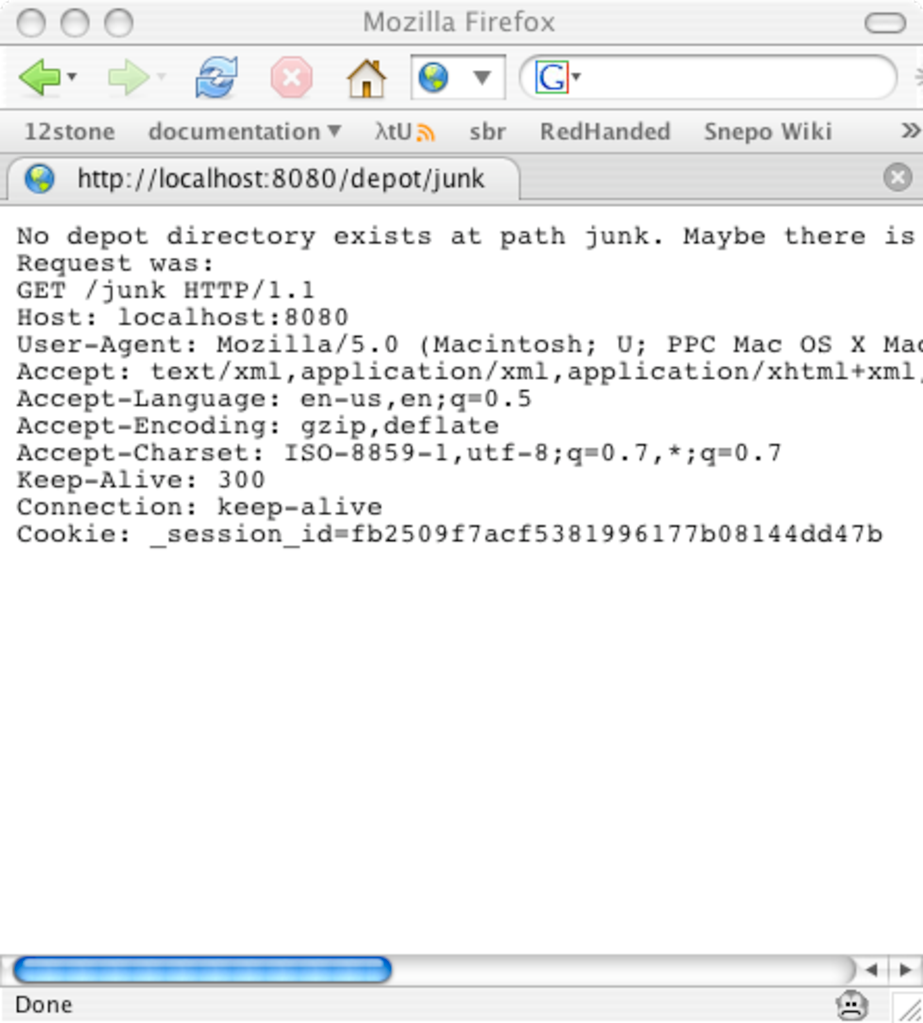
\includegraphics[scale=0.7]{wiki-tutorial-images/wiki-screenshot-404.pdf}
\end{center} 

\paragraph{}
Note that if you are using FireFox the output may not display in the
browser but you will be prompted to download a text file. 
\pagebreak

\section{Building the Wiki}
\pullquote{ 

  \textbf{CAUTION: COPY-PASTING FROM THE PDF DOESN'T ALWAYS WORK}. The
  typesetting system that we use is brilliant for creating nice print
  documents, however some characters will not paste properly and may
  leave you scratching your head as to why the code doesn't
  work. Watch out for quotes (single and double) and special
  characters. If you want to save typing the source files are
  available in your install directory under \texttt{web/wiki}

}
\paragraph{}
Now that depot is running let's build that wiki. Start by putting
together a bit of HTML for your wiki to live in.

\begin{Verbatim}[frame=single]
<html>
  <head>
    <script language="javascript" 
            src="../lib/prototype-1.4.0.js"></script>
    <script language="javascript" 
            src="../lib/depot-client.js"></script>
    <script language="javascript">
      <!-- Wiki code to go here -->
    </script>
  </head>
  <body onload="">
    <h1>The Wiki of the 3 Renaldos</h1>
    <div id="page"></div>
    <a id="edit-link" 
       href="javascript:void;" onclick="">edit</a>
    <div id="revs"></div>
  </body>
</html>
\end{Verbatim}

\paragraph{}
We can call this file \texttt{wiki.html} and place it under the folder
\texttt{<WORKSPACE>/web/wiki-tut/}.

\paragraph{}
Cozy enough, let's look at what we just did: two script tags include
the required javascript files,
\texttt{prototype-1.4.0.js}\footnote{Prototype is an Open Source
  Javascript library freely available from
  http://prototype.conio.net. It is included in the depot
  distribution.} and \texttt{depot-client.js}. These contain library
functions you'll need to store and retrieve things from depot. The
third script tag is where we'll put all of the wiki code.

\paragraph{}
We've added a couple of \texttt{div} tags with ids of
``\texttt{page}'' and ``\texttt{revs}''. The \texttt{page}
\texttt{div} will contain all of the wiki content, \texttt{revs div}
will show the number of revisions that have been made to the page. The
\texttt{edit-link} anchor tag will trigger a page edit, replacing the
content with a textarea for editing.

\paragraph{}
Wikis, as we all know, map a URL to a user generated page. Our Three
Renaldos are quite happy with the format: 

\codeblock{http://localhost:8080/wiki/wiki.html?PageName}

\paragraph{}
Where \textit{PageName} is the CamelCase name of a wiki page. We'd
like to make each wiki page a depot directory and the entries in that
directory will contain the text of the page, one entry for each
edit. That way we can dig through the sordid past of each page. 

\begin{Verbatim}[frame=single]
var wikiPrefix = "/depot/com/snepo/exmples/wiki";
var urlValue   = document.URL.split("?");
var pageName   = "";
if(urlValue[1]) {
  pageName          = urlValue[1];
} else {
  document.location = document.location + "?HomePage"
}

var pageUrl    = wikiPrefix + "/" + pageName;
var page       = new Depot.Object(pageUrl);
\end{Verbatim}

\paragraph{}
First we decide on a prefix for our wiki directory. Depot directory
names must start with \texttt{/depot/} and can't contain spaces or
special characters. Now we extract the value after the ``?'' to
determine the page name. Also note the \texttt{if} statement. If we
are not at a URL that matches our pattern the user is redirected to
the ``HomePage'' page. We combine the prefix and the page name, using the
result to initialise a \texttt{Depot.Object}\footnote{see ``The
  Depot.Object'' on page \pageref{depot.object} for more information
  on available functions and events}:

\pagebreak

\codeblock{http://localhost:8080/wiki/wiki.html?HomePage}

would initialize the \texttt{page} variable with a directory URL of:

\codeblock{/depot/com/snepo/examples/wiki/HomePage}

\paragraph{}
Now it's time to assign event handlers to the \texttt{page}.

\begin{Verbatim}[frame=single]
page.onNotFound  = newPage;
page.onGet       = populatePage;
page.onCreate    = function() {page.getLast();}
\end{Verbatim}
% page.onException = function() {document.location.reload(false);}
\paragraph{}
Each time a command is sent to depot an event is triggered when that
command completes. Trying to read from an empty directory, for
example, will trigger the \texttt{onNotFound} event. Reading a
directory will trigger the \texttt{onGet} event and so on. Above we
have assigned default handlers for the following events: 

\snepolistbox{

\item \texttt{onNotFound} -- A function called \texttt{newPage} will
  be called when a directory cannot be found. This will set up a form
  in the \texttt{page div} so that the user create a new wiki page.

\item \texttt{onGet} -- The function \texttt{populatePage} will get the
  most recent version of the page and display it in the \texttt{page
    div}

\item \texttt{onCreate} -- We assigned an anonymous function that
  calls \texttt{getLast} when new content is added.

% \item \texttt{onException} -- This handler is called whenever there is
%   an exception getting data from the server. This generally happens
%   when there there is an interruption (like somebody hitting the
%   refresh button constantly). The anonymous function that we assign
%   just tells the browser to reload the page and try again.

}

\begin{Verbatim}[frame=single]
function newPage(response, headers) {
  $('edit-link').display = 'none';
  $('page').innerHTML    = 
        "<form><textarea cols='40' rows='20'" +
        "id='edit-wiki'></textarea> " + 
        "<br /><input type='submit' value='save'" + 
        "onclick='createWikiPage(); return false;'/></form>";
}

function populatePage(response, headers) {
  $('page').innerHTML    = response.data;
  $('edit-link').display = 'visible'; 
}

function createWikiPage() {
  page.newDirectory({onCreate: savePage});
}
function savePage() {
  page.create($('edit-wiki').value);
}
\end{Verbatim}

 
... and in the HTML
\begin{Verbatim}[frame=single]
<body onload="page.getLast();">
\end{Verbatim}

Open your browser and go to
\url{http://localhost:8080/wiki/wiki.html}. You should be
presented with a form:

\begin{center}
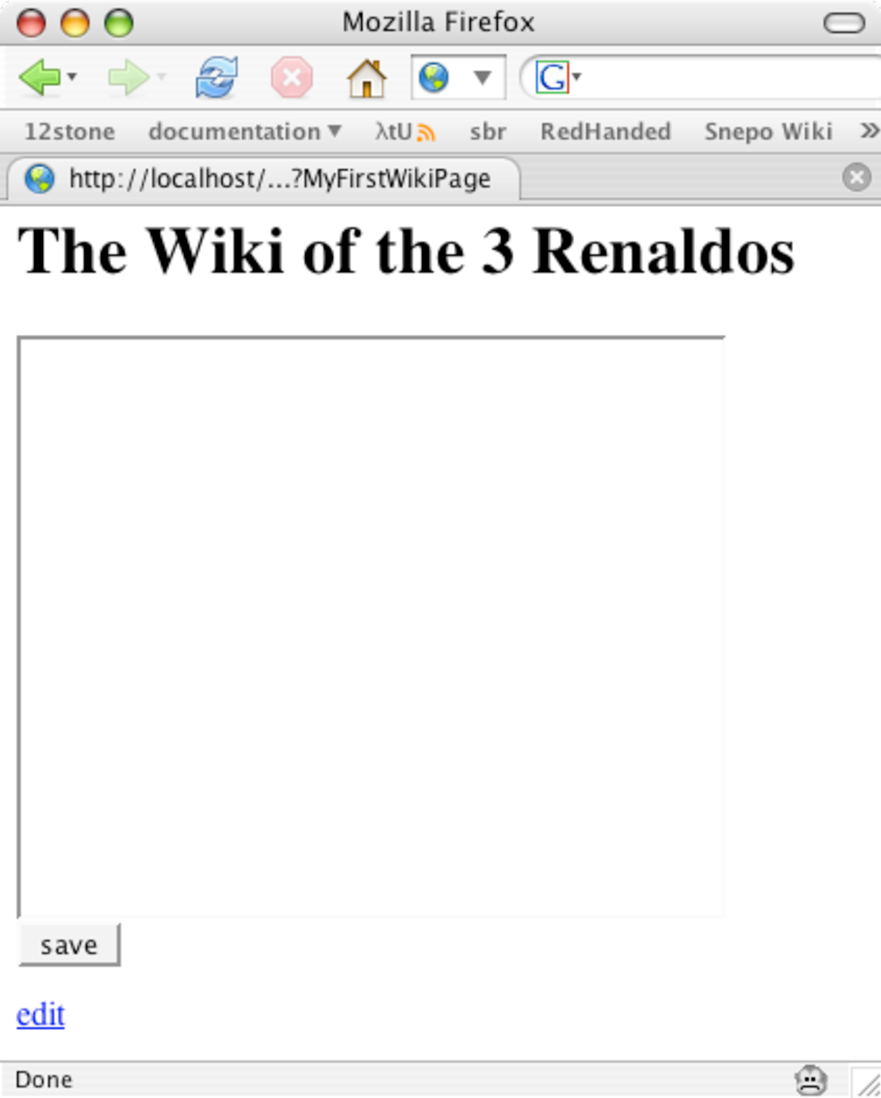
\includegraphics[scale=0.70]{wiki-tutorial-images/wiki-screenshot-1.pdf}
\end{center}
Type some text and hit ``save'': 

\begin{center}
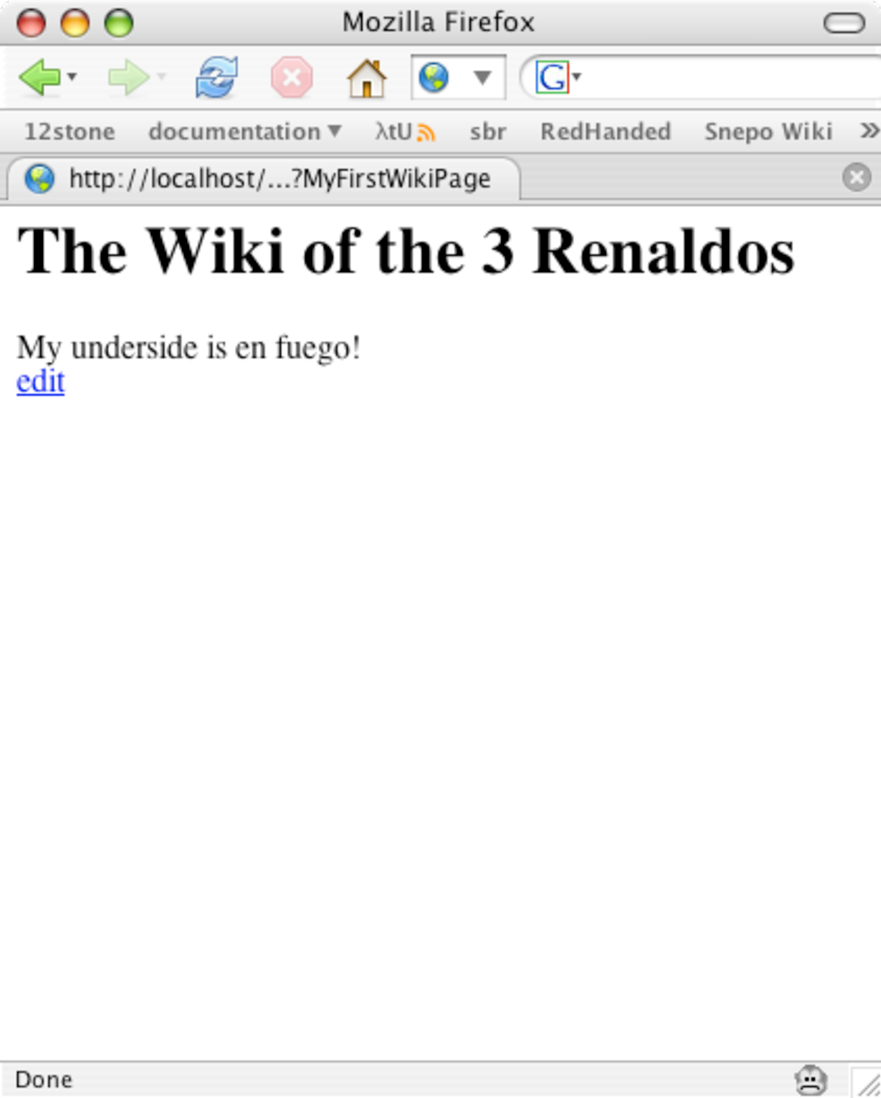
\includegraphics[scale=0.70]{wiki-tutorial-images/wiki-screenshot-2.pdf}
\end{center}

Yeeehaw! You now have a working 1 page wiki. It's not all that Lumberg
asked for but it's getting there. Lets look at what those functions
accomplished:

\snepolistbox {

\item \texttt{newPage} -- This preps us to create a new page by
  putting a form into the \texttt{page div}. Note that the submit
  button in the form calls \texttt{createWikiPage} on click.

\item \texttt{populatePage} -- The handler for \texttt{onGet}, this sets
  the \texttt{page}'s \texttt{innerHTML} property to the value of the
  data returned in the \texttt{response}.

\item \texttt{createWikiPage} -- Calls \texttt{newDirectory} but
  temporarily overrides the handler for \texttt{onCreate} with the
  \texttt{savePage} function. Overrides can be passed through for any
  event, they allow you to temporarily change the default action. In
  this case its necessary because creating a new directory and adding
  an entry in a directory both trigger the same \texttt{onCreate}
  event.

\item \texttt{savePage} -- Creates a new entry with the value of the
  \texttt{wiki-edit textarea}

 }

\paragraph{}


All in all you have a 1 page wiki in about 32 lines of Javascript. I
suppose you'll want to be editing it and adding all of the fancies
that you were promised back in paragraph 2? Keep reading, your pizza
is almost here.

\chapter{Features, Features, Features!}
\paragraph{}
The first feature we'll need to add is the ability to edit a page once
it's been created. This is sort of important. Let's add the following
to the \texttt{edit-link} anchor tag:

\begin{Verbatim}[frame=single]
    <a id="edit-link" href="javascript:void;"
       onclick="editPage();return false;">edit</a>
\end{Verbatim}

And the functions \texttt{editPage} and \texttt{populateEditBox}.

\begin{Verbatim}[frame=single]
function editPage() {
   $('page').innerHTML = 
    "<form><textarea  cols='40' rows='20' id='wiki-edit'>" + 
    "</textarea><br /><input type='submit'" +
    " onclick='return savePage();'" +
    "value='save' /></form>";
   page.getLast({onGet: populateEditBox});
}
function populateEditBox(response, headers) {
  $('wiki-edit').value = response.data;
}
\end{Verbatim} 

\paragraph{}
The \texttt{editPage} function does two main things, first it replaces
the page div with a text area and a submit button much like
\texttt{newPage}. Then it makes a call to \texttt{page.getLast}. We
are overriding the \texttt{onGet} handler in the same way we did
earlier for \texttt{newDirectory}. Remember that overriding defaults
in this way only affects the current call that is being made and won't
change the defaults themselves. The \texttt{populateEdit} callback
sets the text area value

\paragraph{}
Try it out! Now you can edit pages to your hearts

\section{Marty's Trousers}
\paragraph{}
Alright McFly, let's go back in time, all the way back to a few
minutes ago. Add a line to the \texttt{populatePage} function:
\begin{Verbatim}[frame=single]
function populatePage(response, headers) {
  $('page').innerHTML    = response.data;
  $('edit-link').display = 'visible';
  page.size({onGet: showRevs}); // add this line
}
\end{Verbatim}

Now add the following: 
\begin{Verbatim}[frame=single]
function showRevs(response,headers) {
 var prevLink       = "<a href='javascript:void;' " + 
       "onclick='viewPrevious();return false;'>" + 
       "view previous?</a>";
 $('revs').innerHTML =  response.directorySize + 
       " revisions, " + prevLink;
}

function viewPrevious() {
  page.getAll({onGet: showPreviousLinks});
}
function showPreviousLinks(response,headers) {
  var lis = "";
  // check to see if response is an Array
  // queries like getAll return an Array of results 
  // if more than 1 item is in the directory
  if(response.each) {
    var revisionListItems = $A([]);
    responses.each(function(d) {
        revisionListItems.push(makeRevisionListItem(d));
    });      
    lis = revisionListItems.join("");
  } else {
    lis = makeRevisionListItem(responses);
  }
  $('page').innerHTML = "<ul>" + lis + "</ul>";
}
function makeRevisionListItem(revResponse) {
  return "<li><a href='javascript:void;' " + 
	 "onclick='page.get(" + 
          revResponse.objectId + 
          "); return false'> Revision " + 
	  revResponse.objectId + "</a></li>";
}
\end{Verbatim}
%$

The \texttt{size} function gets the number of entries in a depot
directory, we pass it the \texttt{showRevs} function as a handler for
\texttt{onGet}. Now we have three functions to add to implement our
time travelling Delorean:


\snepolistbox{
  \item \texttt{showRevs} -- adds a link to view previous versions of the
    wiki entry, on click it calls \texttt{viewPrevious}

  \item \texttt{viewPrevious} -- which retrieves all the entries in the
    current directory 

  \item \texttt{showPreviousList} -- the callback for viewPrevious which
    loops through the results. The \texttt{getAll} command returns
    everything in a directory. If there are more than one results
    returned the \texttt{responses} variable will be an Array of
    response items, otherwise it will be a normal response item.

  \item \texttt{makeRevisionListItem} -- is a utility function to
    return an HTML \texttt{li} tag with a link that calls \texttt{get}
    on a revision \texttt{objectId}

 }

\paragraph{}
 Now refresh your page and check that you can see the following screen
 by hitting the \textit{view previous} link.

\begin{center}
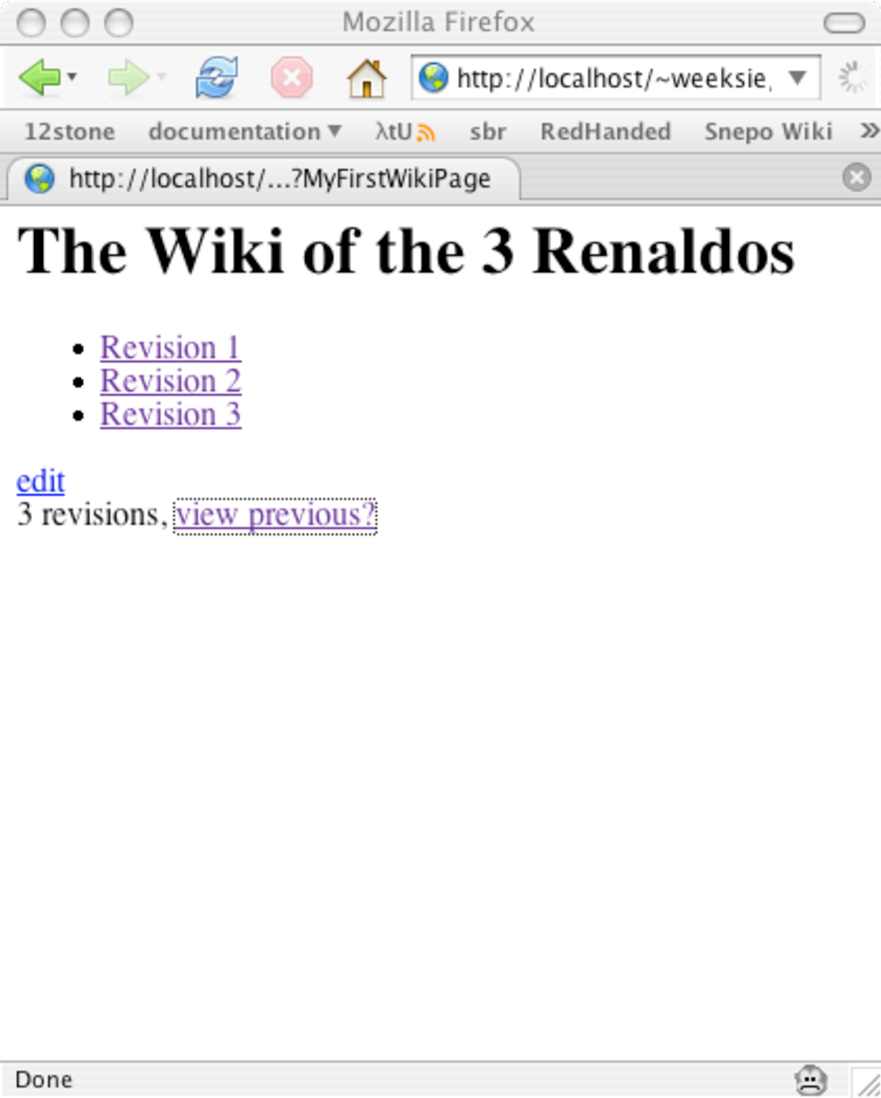
\includegraphics[scale=0.70]{wiki-tutorial-images/wiki-screenshot-4.pdf}
\end{center}


\section{Wacky Wiki Words}

\paragraph{}
Now, just a little more spice to complete things, wiki words! 


\begin{Verbatim}[frame=single]
var wikiWord  = /\b(([A-Z][a-z]+){2,})\b/g;
function wikiLink(text) {
  return text.replace(wikiWord, "<a href='?$1'>$1</a>");
}
\end{Verbatim}

And one minor change to the \texttt{populatePage} function

\begin{Verbatim}[frame=single]
function populatePage(response, headers) {
  $('page').innerHTML    = wikiLinks(response.data); 
  $('edit-link').display = 'visible';
  page.size({onGet: showRevs});
}
\end{Verbatim}

\begin{center}
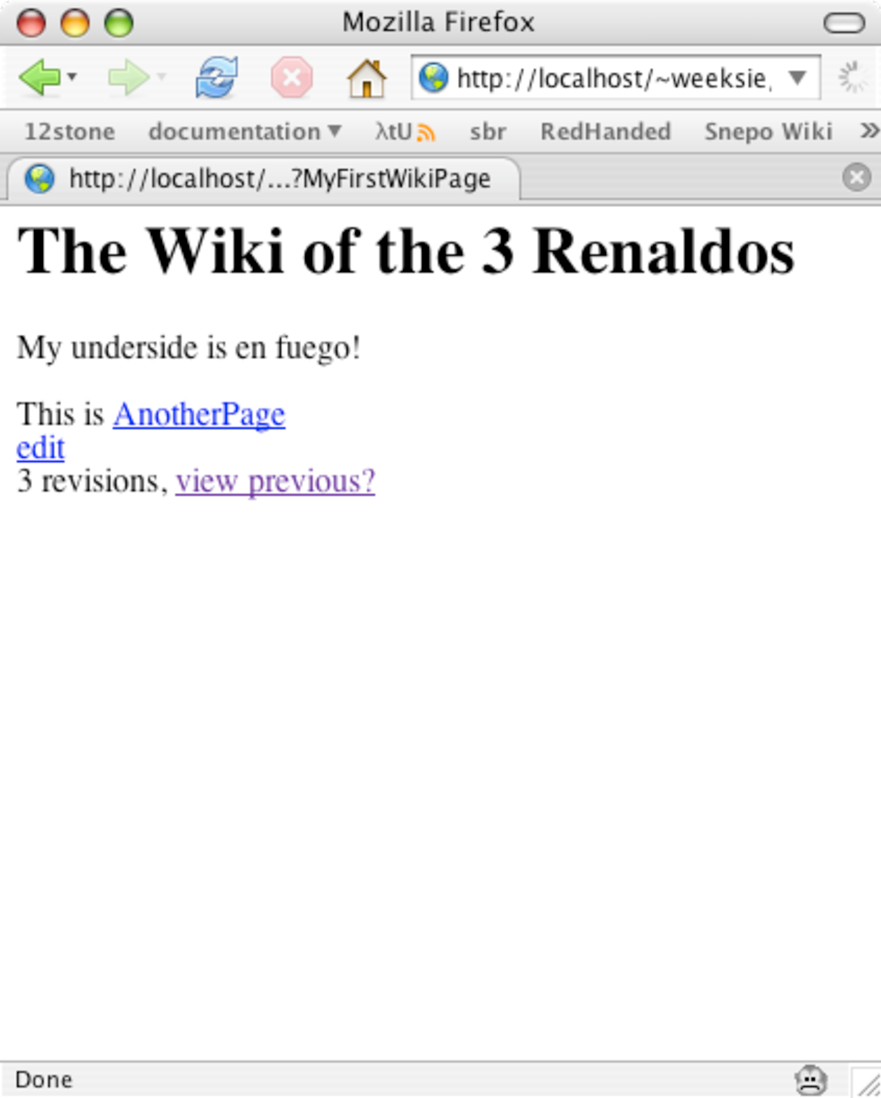
\includegraphics[scale=0.70]{wiki-tutorial-images/wiki-screenshot-3.pdf}
\end{center}

There you have it! A few minutes and you've got a working, versioned
wiki. The entire code for the finished product under the
\texttt{web/wiki} directory in your Depot install. Now you can brag to
all of your friends that you built an Ajax wiki in under 30 minutes
without having to use PHP, databases. And you haven't been attacked by
wild cats, which is a plus.



\begin{appendices}


\chapter{The Depot.Object}
\label{depot.object}

\paragraph{}
Depot stores objects in directories, to represent a connection to a
directory we need an instance of a \texttt{Depot.Object}. The
\texttt{Depot.Object} takes an absolute path that points at a depot
url, remember that you will need to prefix your path with
\texttt{/depot}.

\codeblock{ var page = new Depot.Object("/depot/hot/monkeys");}

\paragraph{}
The Depot.Object has several commands that can be used to store
and retrieve data from a directory.

\snepolistbox{

\item \texttt{get} retrieves an object by its id.
\item \texttt{getAll} retrieves all objects in a directory
\item \texttt{getFirst} retrieves the first object stored in a directory
\item \texttt{getLast} retrieves the last object stored in a directory
\item \texttt{getRange} retrieves an object between two boundary ids
  (e.g. from 1 to 30 inclusive) 
\item \texttt{size} retrieves the number of entries stored in the directory
\item \texttt{newDirectory} creates a new directory
\item \texttt{restoreDirectory} brings a removed directory back
\item \texttt{removeDirectory} removes a directory
\item \texttt{destroyDirectory} irreversably destroys a directory
\item \texttt{create} adds an entry to the directory
\item \texttt{remove} deletes a directory entry
\item \texttt{executeQuery} \textbf{Only for hacking} this allows raw
  URL queries to be sent to the depot server. This is for expirimenting with depot
}

\paragraph{}
The result of method calls to \texttt{Depot.Object} are accessed with
callback functions:

\snepolistbox {
\item \texttt{onGet}  a \texttt{get} command is
  successful 

\item \texttt{onCreate} a new object was created (either
  a directory or an entry in a directory)

\item \texttt{onDelete} an object was removed or destroyed

\item \texttt{onNotFound} an action couldn't be completed because the
  directory or object does not exist.

\item \texttt{onServerError} an error has occured on the depot server.

\item \texttt{onException} an error has occured inside Javascript code.

 }

\paragraph{}
All of these functions and events are explained in more detail both on
the \url{http://depot.snepo.com} site and in the \texttt{users.pdf}
document.


\end{appendices}


\end{document}
